\chapter{Stakeholderanalyse}
Für die STH App sind Stakeholder aus verschiedenen Bereichen vorhanden. Die Applikation erstrebt einen großen Einfluss auf die Sportindustrie und das speziell auf den Prozess des Anwerbens von neuen Talenten durch Vereine in unterschiedlichen Größen. Deshalb ist eine Stakeholderanalyse besonders wichtig, um die verschiedenen Gruppen an Interessenten identifizieren zu können. Für die Analyse werden folgende Gruppen an Stakeholdern betrachtet: Interne-, Externe-, Community- und Technische-Stakeholder. 

\noindent
Die Stakeholderanalyse wurde mit einem konkreten Vorgehen erstellt. Zuerst wurde erneut die Größe und Auswirkung der Applikation betrachtet.
Dabei ist es auch wichtig, die Zielsysteme iOS und Android nicht außer Acht zu lassen, um konkrete Benutzergruppen definieren zu können. Innerhalb des Projektteams wurde in einem Meeting gemeinsam festgelegt, welche Stakeholder für die STH-App infrage kommen.

\section{Management}
Zunächst wurden die internen Stakeholder und das Management betrachtet.
Dabei wurde das Projektteam und das Hochschulpersonal identifiziert. Das Projektteam der STH-App ist am Erfolg der Applikation interessiert, da das Projektteam sowohl an der Organisation und an der Entwicklung der STH-App beteiligt ist.

\section{Partner / Stakeholder}
Zu den Partnern und Stakeholdern hat das Projektteam folgende Personengruppen erkannt. Amateursportler, Sportagenturen, Manager, Vereine und Scouts sind externe Interessensgruppen, die den Erfolg der Applikation als relevant betrachten. Diese Gruppen an Personen haben einen direkten Bezug zur Applikation und stellen die zukünftigen Anwender dar. Das Interesse am Verlauf und Erfolg der Applikation ist in diesen Gruppen stark vertreten, da hier ein Mehrwert für all diese Gruppen erzielt werden kann. Aus der Hülle der Anwender heraus wurden weitere Stakeholdergruppen vom Projektteam erkannt.

\noindent
Eine weitere relevante Gruppe ist die Community hinter den Anwendern. Dazu zählen Sportmedien und große Sportverbände, die keinen direkten Bezug zur Applikation haben, aber dennoch am Einfluss der STH-App in ihren Sportbereichen interessiert sind. Sportmedien werden über die Bekanntmachungen von neuen Verträgen über die STH-App berichten. Sportverbände sind an großen und performanten Sportvereinen interessiert, welche über die STH-App die Kommunikation für Spielertransfers durchführen können.

\section{Externe Partner}
Zu den Externen Stakeholdern wurden zudem die technischen und rechtlichen Interessensgruppen erkannt.Innerhalb der STH-App werden persönliche Daten wie z.B. Name, Vorname, Wohnort, PLZ und die E-Mail hinterlegt. Die personenbezogenen Daten unterliegen strikten Regeln durch die Gesetzgebung der Datenschutz-Grundverordnung.
Datenschutzbeauftragte werden ein großes Interesse an der korrekten Datenhaltung der STH-App nach der Veröffentlichung der Anwendung haben. Zudem sind die App-Stores wie der Google Play Store und der Apple App Store daran interessiert, dass diese Gesetzgebungen eingehalten werden und zudem auch die Richtlinien und Vorgaben der Stores eingehalten werden. Die Applikation muss für eine Veröffentlichung auf diesen Plattformen diesen Regelungen strikt folgen.
Deshalb zählen diese Firmen und Personengruppen zu einem weiteren großen Teil der Stakeholder.\newline

\noindent
Die Stakeholderanalyse zeigt zum aktuellen Zeitpunkt der STH-App eine Vielzahl an Interessensgruppen auf, die am Erfolg oder an dem Verlauf des Projektes STH-App interessiert sind.


\section{Grafische Darstellung Stakeholderanalyse}

In der folgenden Abbildung sind die Stakeholdergruppen und deren Abhängigkeiten aufgezeichnet.
\begin{figure}[H]
	\setcounter{figure}{4} 
	\caption[Stakeholderanalyse]{Stakeholderanalyse}
	\centering
	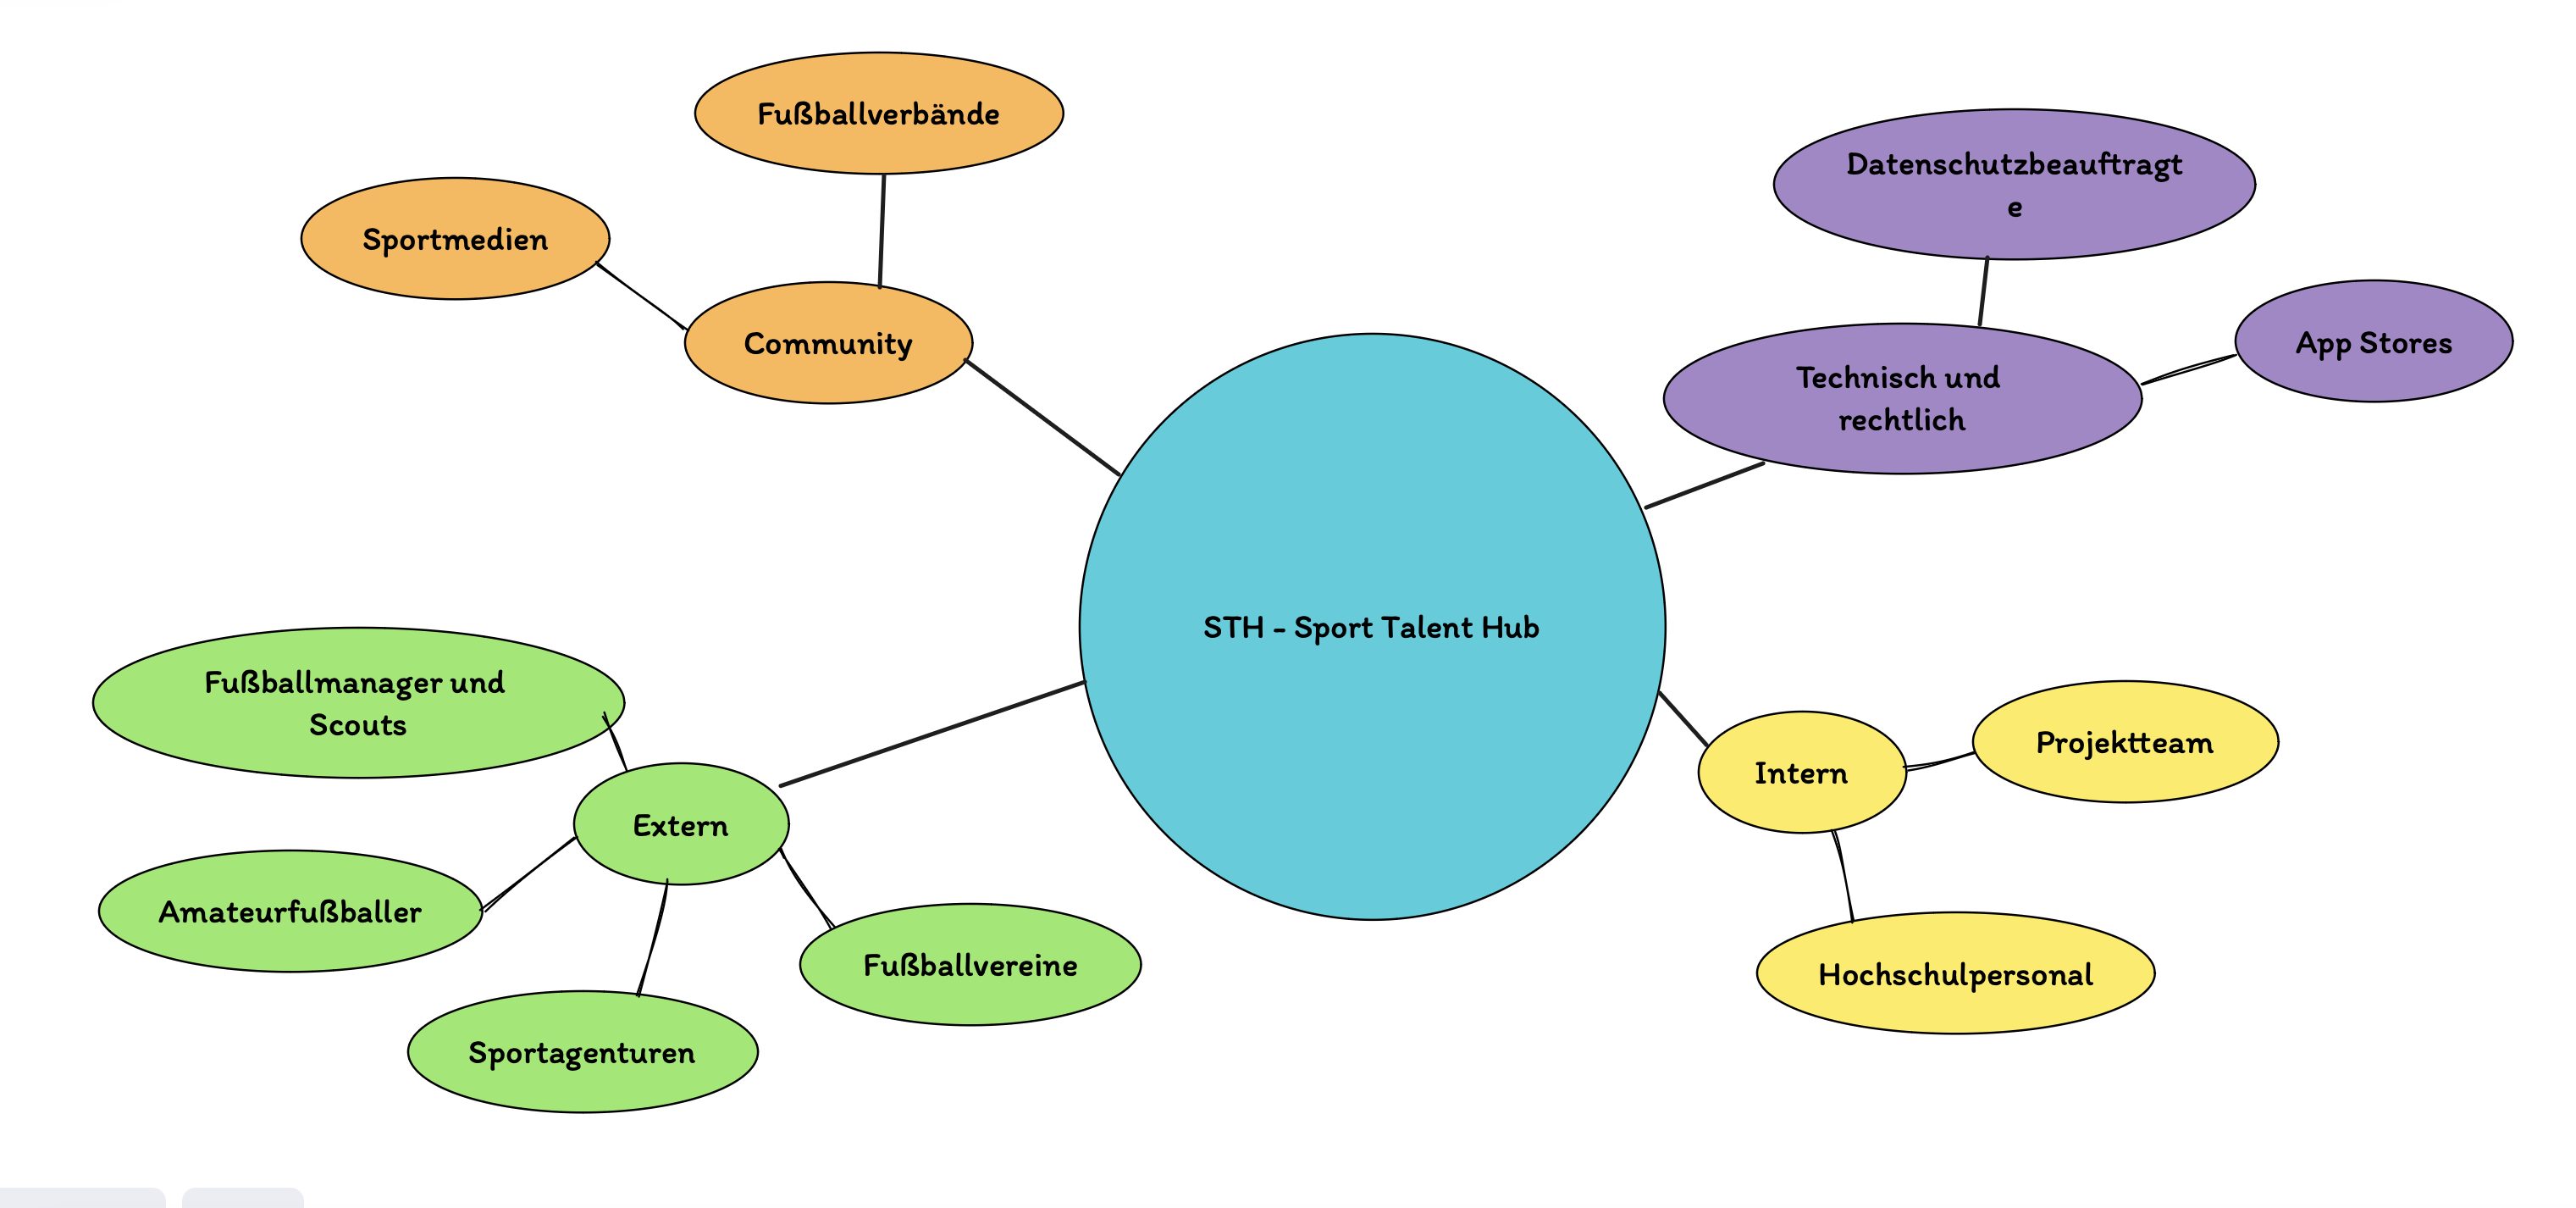
\includegraphics[width=0.9\textwidth]{assets/figures/Stakeholderanalyse.png}
	\begin{flushleft}
		Quelle: Eigene Darstellung
	\end{flushleft}
\end{figure}


